\section{Технический проект}
\subsection{Общая характеристика архитектуры решения}

Графический движок представляет собой кроссплатформенное приложение для визуализации трёхмерных сцен, построенное на следующих ключевых компонентах:

\begin{itemize}
    \item подсистема управления окнами (SDL2);
    \item графический конвейер (OpenGL 3.3);
    \item подсистема загрузки ресурсов (текстуры, шейдеры);
    \item менеджер сцен и объектов.
\end{itemize}

Движок спроектирован как модульная система, позволяющая расширять функционал без изменения ядра.

\subsection{Обоснование выбора технологий}

\subsubsection{Язык программирования C++}

В качестве основного языка разработки выбран C++ -- высокопроизводительный компилируемый язык, обеспечивающий прямой доступ к API библиотек. Его кроссплатформенная природа позволяет компилировать движок под различные операционные системы без изменения исходного кода. Современные стандарты C++ предоставляют необходимые средства для эффективной работы с памятью и многопоточностью, что критично для графических приложений.

\subsubsection{Система сборки CMake}

В качестве системы управления сборкой в проекте применяется CMake, что обусловлено его гибкостью и широкой поддержкой в индустрии разработки программного обеспечения. Использование CMake позволяет централизованно описывать структуру проекта, автоматически находить и подключать сторонние библиотеки, а также формировать корректные проекты для различных платформ и сред разработки. Современные стандарты CMake делают сборочный процесс прозрачным и легко масштабируемым: добавление новых исходных файлов или зависимостей не требует ручных изменений для каждой платформы.

Использование подобной системы минимизирует вероятность ошибок, связанных с различиями между платформами, и ускоряет процесс разработки.

\subsubsection{Компилятор GCC}

Для компиляции движка был выбран бесплатный компилятор с открытым исходным кодом GCC (GNU Compiler Collection), обеспечивающий возможность компиляции C и C++ кода с поддержкой современных стандартов. GCC по-умолчанию поддерживается только на операционной системе Linux, но имеет возможность компиляции под Windows с помощью MinGW.

\subsubsection{Набор инструментов разработки MinGW}

Для сборки и запуска проекта на платформе Windows используется набор инструментов разработки MinGW (Minimalist GNU for Windows), который предоставляет среду для работы с GCC. Он также обеспечивает совместимость с другими инструментами Linux, что облегчает переносимость кода между платформами, а также позволяют использовать единые скрипты сборки и тестирования.

В процессе разработки данного проекта MinGW показал себя как надёжное и удобное решение для удобной разработки под Windows.

\subsubsection{Библиотека SDL2}

Для взаимодействия с оконной системой используется библиотека SDL2 (Simple DirectMedia Layer), которая абстрагирует платформозависимые особенности создания окон, обработки ввода и работы с аудио. SDL2 была выбрана благодаря своей стабильности, поддержке нескольких платформ и минимальным затратам времени на адаптацию. Библиотека предоставляет простой API для инициализации графического контекста OpenGL и обработки пользовательского ввода.

\subsubsection{Спецификация графического API OpenGL}

Графический конвейер реализован на основе OpenGL 3.3 Core Profile -- кроссплатформенного графического API, поддерживаемого большинством современных видеокарт. Выбор версии 3.3 обусловлен балансом между функциональностью и совместимостью: этот стандарт предоставляет современный конвейер рендеринга с шейдерной моделью, но при этом не требует новейшей аппаратуры.

Для привязки аппаратных функций OpenGL к структурам языка C++ используется загрузочная библиотека Glad.

OpenGL был предпочтен Vulkan и Direct3D ввиду своей универсальности и меньшего порога входа.

\subsubsection{Язык программирования шейдеров GLSL}

GLSL (OpenGL Shading Language) является языком программирования для написания шейдеров, используемых в конвейере рендеринга. Шейдеры позволяют конечным пользователям настраивать различные аспекты визуализации, такие как текстуры, освещение и эффекты, без перекомпиляции основной части программы. Все операции шейдеров выполняются на графическом ускорителе, что обеспечивает высокую производительность.

\subsubsection{Математическая библиотека GLM}

Библиотека GLM (OpenGL Mathematics) предоставляет математические функции и типы данных, специфичные для компьютерной графики:

\begin{itemize}
    \item операции с векторами и матрицами (произведение, сложение, вычитание);
    \item трансформации (перемещение, вращение, масштабирование);
    \item пространственных преобразований (нормализация, проекции).
\end{itemize}

GLM применяется в движке для упрощения таких действий, как расчёт матриц модели, вида и проекции, преобразование координат и управление камерой и перспективой.

Библиотека была выбрана благодаря полной совместимости с OpenGL, оптимизированным SIMD-операциям и удобному синтаксису, аналогичному GLSL.

\subsection{Архитектурные компоненты системы}

Диаграмма компонентов (рис. \ref{comp:image}) отражает физическую и логическую структуру графического движка. Архитектура системы построена по принципу разделения ответственности, где каждый компонент инкапсулирует строго определённую функциональность.

\afterpage{
  \begin{landscape}
    \begin{figure}[p]
      \centering
      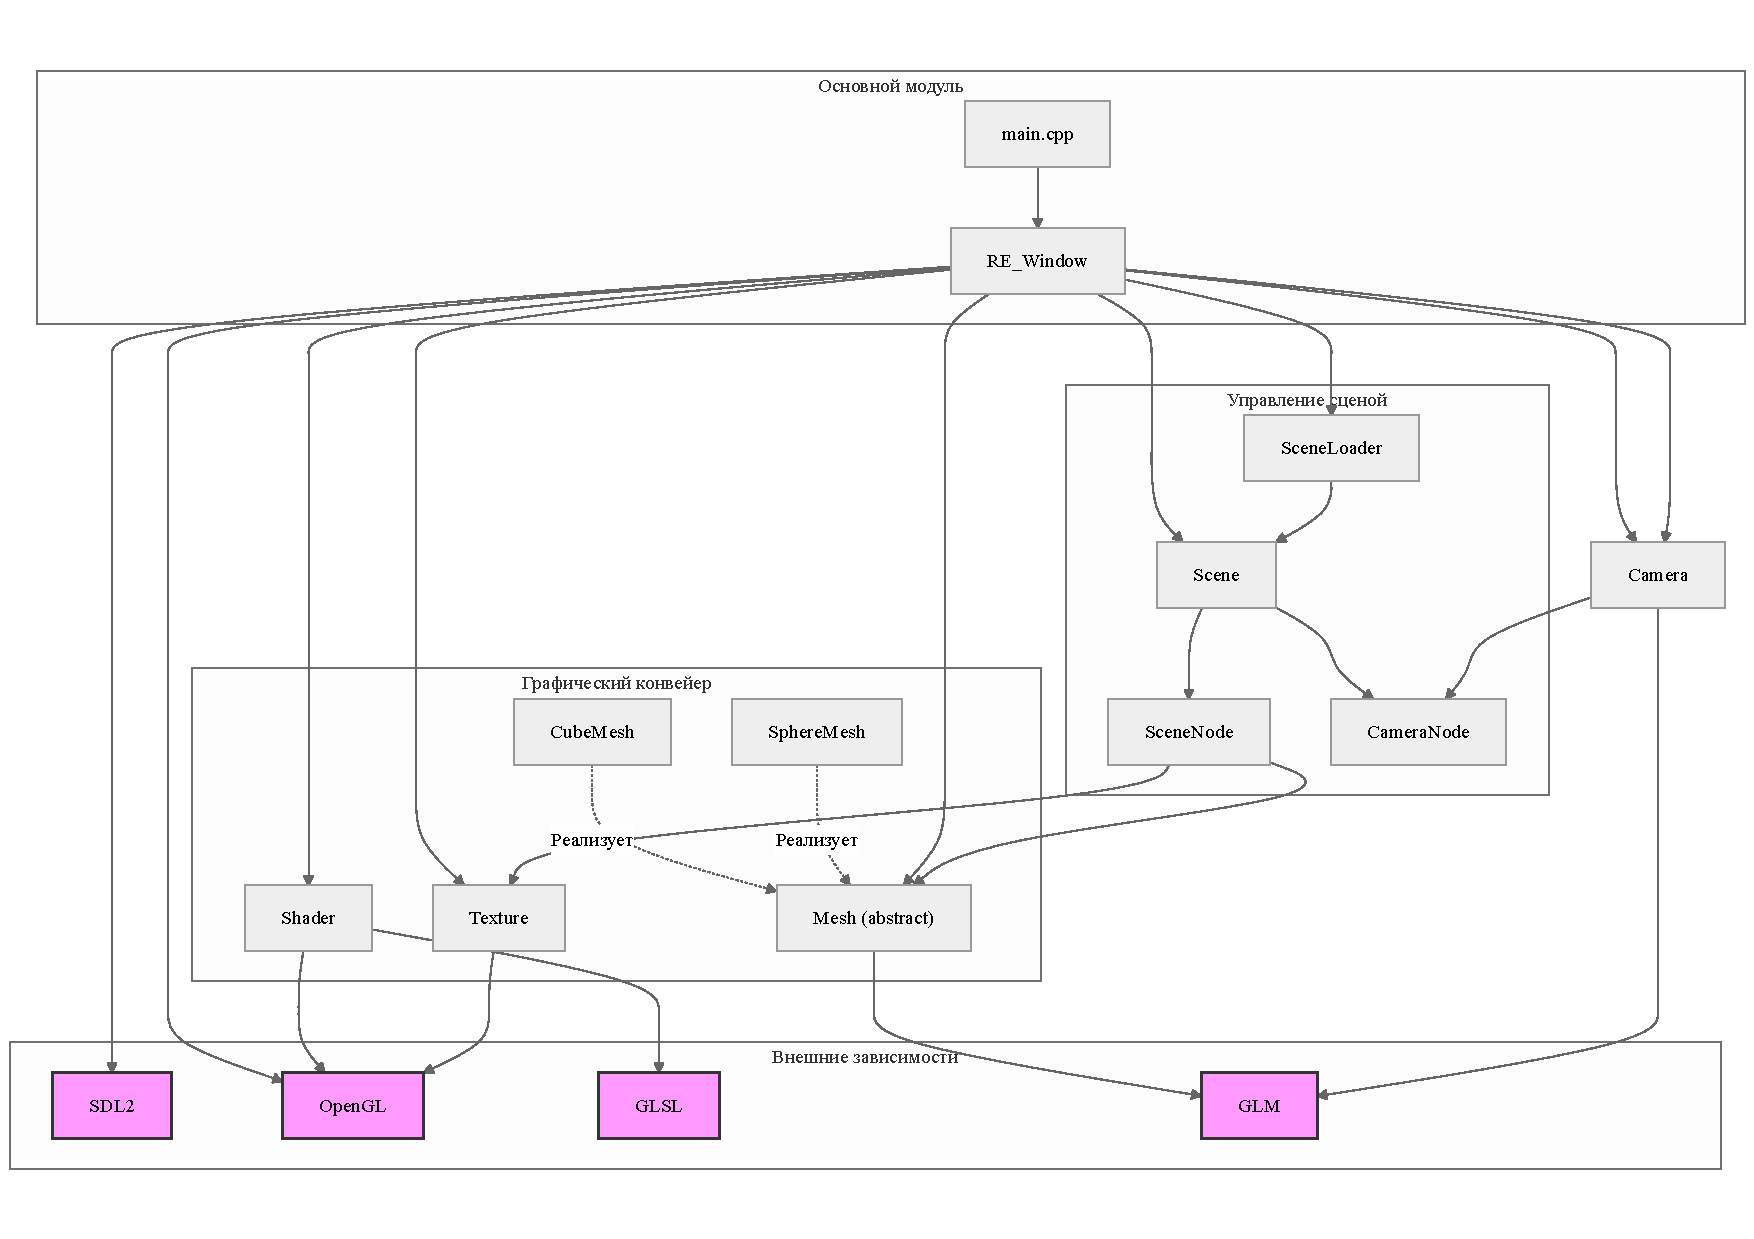
\includegraphics[width=1.6\textwidth]{comp.pdf}
      \caption{Диаграмма компонентов движка с последовательностью взаимодействия}
      \label{comp:image}
    \end{figure}
  \end{landscape}
}

\subsubsection{Состав компонентов}

Основные модули системы включают:

\begin{enumerate}
    \item Window -- компонент управления окном, реализующий:

    \begin{itemize}[itemindent=\parindent,leftmargin=\parindent]
        \item инициализацию окна;
        \item обработку ввода;
        \item обработку событий.
    \end{itemize}

    \item Renderer -- компонент управления конвейером рендеринга, реализующий абстракцию над API OpenGL. Обеспечивает:

    \begin{itemize}[itemindent=\parindent,leftmargin=\parindent]
        \item инициализацию контекста OpenGL;
        \item загрузку шейдеров;
        \item управление сценой;
        \item отрисовку сцены.
    \end{itemize}

    \item Scene -- подсистема работы со сценой:

    \begin{itemize}[itemindent=\parindent,leftmargin=\parindent]
        \item хранит коллекцию объектов (SceneNode) и управляет их состоянием;
        \item хранит камеру и параметры освещения;
        \item поддерживает цвет неба (skyColor), параметры направленного и точечных источников света (DirLight, PointLight), а также масштабируемое количество источников света.
    \end{itemize}

    \item InputHandler -- компонент обработки пользовательского ввода:

    \begin{itemize}[itemindent=\parindent,leftmargin=\parindent]
        \item предоставляет интерфейс для регистрации callback-функций на нажатие, удержание и отпускание клавиш;
        \item поддерживает обработку событий мыши (движение, нажатие, прокрутка);
        \item хранит состояния клавиш и мыши;
        \item обеспечивает получение текущей позиции и относительного перемещения мыши.
    \end{itemize}

    \item Графический конвейер (неявный компонент):

    \begin{itemize}[itemindent=\parindent,leftmargin=\parindent]
        \item Shader -- управление шейдерными программами (вершинный/фрагментный);
        \item Texture -- загрузка, генерация и привязка текстурных объектов;
        \item Mesh -- хранение геометрических данных (VBO/VAO/EBO).
    \end{itemize}

    \item Camera -- компонент управления видами, реализующий:

    \begin{itemize}[itemindent=\parindent,leftmargin=\parindent]
        \item расчёт матриц вида и проекции;
        \item преобразование координат;
        \item управление параметрами отображения (позиция, углы, FOV);
        \item относительное перемещение и вращение;
        \item получение и установка углов поворота.
    \end{itemize}
\end{enumerate}

\subsubsection{Взаимодействие компонентов}

Последовательность работы системы (рис. \ref{comp:image}) реализуется следующим образом:

\begin{enumerate}
    \item Инициализация:

    \begin{itemize}[itemindent=\parindent,leftmargin=\parindent]
        \item Renderer создаёт графический контекст;
        \item Shader компилирует шейдерные программы;
        \item SceneLoader загружает начальную сцену.
    \end{itemize}

    \item Главный цикл рендеринга:

    \begin{itemize}[itemindent=\parindent,leftmargin=\parindent]
        \item обновление матриц вида в Camera;
        \item передача uniform-переменных в шейдеры;
        \item формирование вершинного буфера объектов сцены из вектора SceneNode;
        \item отрисовка объектов сцены с учётом их:

        \begin{itemize}[itemindent=\parindent,leftmargin=\parindent]
            \item геометрии (Mesh);
            \item текстуры (Texture);
            \item шейдеров (Shader).
        \end{itemize}

        \item вывод результата через Renderer;
        \item обработка пользовательского ввода Renderer и передача его значений в Camera;
        \item повтор цикла до выхода из программы.
    \end{itemize}
\end{enumerate}
